\chapter{Zobecněné Paretovo rozdělení}\label{chap:gpd}
\#TODO

\begin{equation}
    F_u(x)=P(X-u \leq x,X>u)=\frac{F(u+x)-F(x)}{1-F(x)}
\end{equation}

\begin{equation}
    F_u(x)=P(X-u \leq x,X>u)=\frac{F(u+x)-F(x)}{1-F(x)}
\end{equation}


\begin{equation}
  f_{(\xi,\mu,\sigma)}(x)=\begin{cases}
    \frac{1}{\sigma}\Bigg(1+\frac{\xi(x-\mu)}{\sigma}\Bigg)^{\Big(-\frac{1}{\xi}-1\Big)} & \text{for $\xi \neq 0$},\\
    \exp \Big(-\frac{x-\mu}{\sigma}\Big) & \text{for $\xi = 0$}.
  \end{cases}
\end{equation}


\begin{equation}
  F_{(\xi,\mu,\sigma)}(x)=\begin{cases}
    1 - \Bigg(1+\frac{\xi(x-\mu)}{\sigma}\Bigg)^{-\frac{1}{\xi}} & \text{for $\xi \neq 0$},\\
    1 - \exp{\Big(-\frac{x-\mu}{\sigma} \Big)} & \text{for $\xi = 0$}.
  \end{cases}
\end{equation}

\begin{figure}
    \centering
    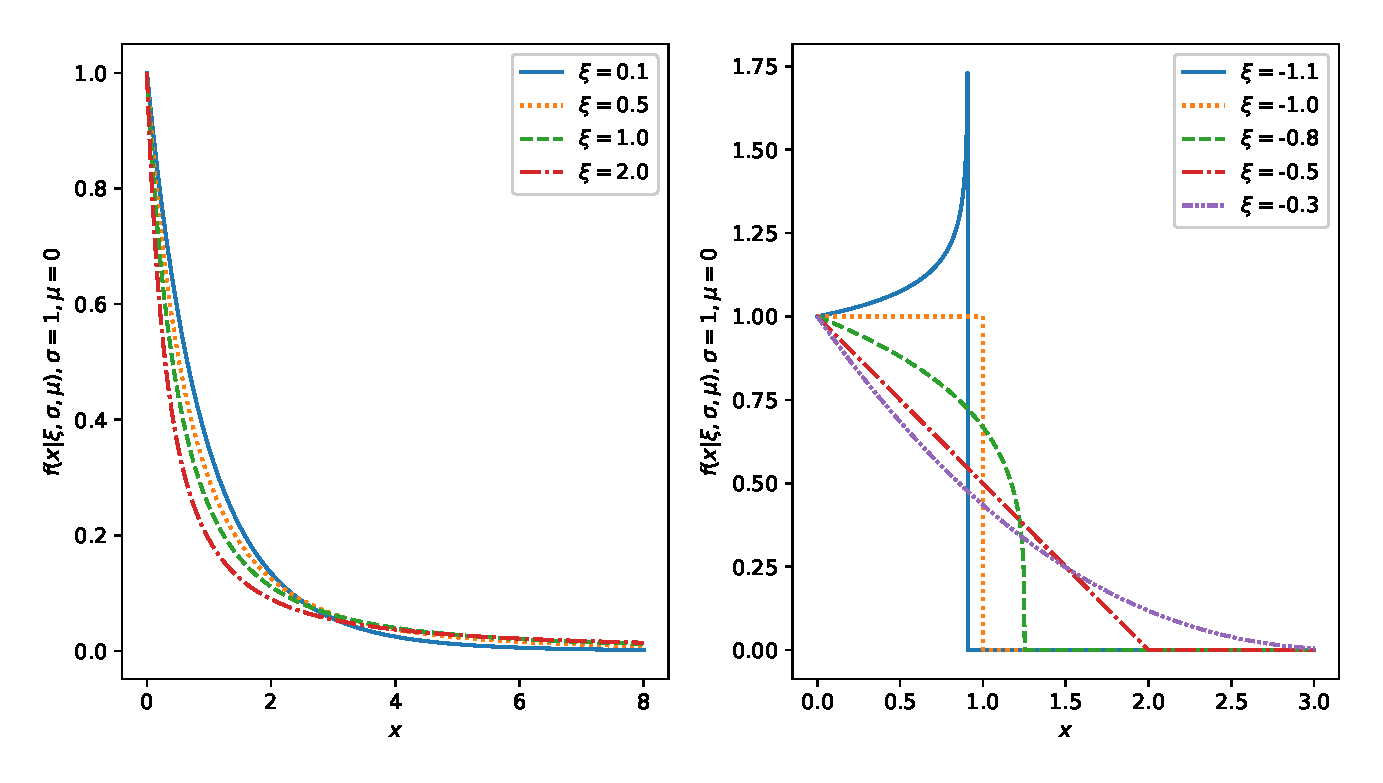
\includegraphics[scale=0.68]{IMG/MDPI/pdfs.eps}
    \caption{\textcolor{red}{GPD probability density function with various parameters $\xi$, and fixed parameters $\sigma=1$, $\mu=0$}}
    \label{fig:gpd_pdfs}
\end{figure}

\section{Metoda Peak-over-Threshold}
Zásadním problémem při hledání parametrů GPD je volba vhodné hodnoty prahu $z$. Metody, které řeší uvedený problém jsou nazývány Peak-Over-Threshold (POT). V případě, že je hodnota prahu $z$ příliš vysoká, mají parametry GPD velkou varianci, protože je existuje pouze příliš málo dat, které zvolenou prahovou hodnotu překročí. Pokud je hodnota prahu $z$ naopak příliš nízká, není aproximace ocasu generujícího rozdělení spolehlivá.  Z tohoto pohledu, je tedy vhodná volba hodnoty prahu $z$ pro kvalitu fitu GPD zásadní. Existuje celá řada metod pro výběr hodnoty prahu (více viz \cite{scarrott2012review}). Některé z metod POT jsou však sami o sobě výpočetně náročné, případně poskytují výsledky, jež musí být vyhodnoceny expertem. Z těchto důvodů nejsou příliž vhodné pro algoritmus detekce novosti, který by vyhodnocoval data v reálném čase. Proto se zdá vhodné využít některé z metod "Rule of Thumb".

 \cite{dumouchel1983estimating,ferreira2003optimising,loretan1994testing} choice of threshold were used. Let $l$ is the number of samples used for GPD fitting and $n_s$ is total number of samples available:
\begin{equation} \label{eq:l1}
    l_1=\ceil[\big]{0.1 \cdot n_s}
\end{equation}
\begin{equation} \label{eq:l2}
    l_2=\ceil[\big]{\sqrt{n_s}}
\end{equation}
\begin{equation} \label{eq:l3}
     l_3=\ceil[\bigg]{\frac{\sqrt[3]{n_s^{2}}}{log(log(n_s))}}
\end{equation}

Note, that we use the highest adaptive weight increments to estimate the GPD parameters. The \textcolor{red}{Peaks-over-threshold (POT)} method is crucial to decide, whether the $|\Delta w_k(k)|$ belongs to set $H_i$ or $L_i$. In section \ref{experiments} there are results with different techniques of threshold choice.

\section{Metody odhadu parametrů zobecněného Paretova rozdělení}
\#TODO